\documentclass[reqno, a4paper]{amsart}
\author{J. Púček, L. Košárková, M. Fuksa}
\usepackage{amsmath}
\usepackage{amssymb}
\usepackage{amsthm}

\usepackage[scale=0.9]{geometry}
\usepackage{mathbbol}

\usepackage[utf8]{inputenc}

\usepackage{subfig}
\usepackage{graphicx}
\usepackage{multicol}
\usepackage[font=small,labelfont=bf]{caption}
\usepackage{graphicx,wrapfig}

%\makeatletter
% \@ifpackageloaded{tensor}% tensor is a package for a better typesetting of tensors
% {
% \renewcommand{\tnsr@Aux}[3][]{%
% \mathpalette{\tnsr@Plt{#1}{#3}}{\mathrm #2}%
% \tnsr@Wrn
% }%\tnsr@Aux
% }{%
% \relax%
% }
% \makeatother


% operators
\DeclareMathOperator{\divergence}{div}
\DeclareMathOperator{\Divergence}{Div}
\DeclareMathOperator{\gradient}{grad}
\DeclareMathOperator{\Gradient}{Grad}
\DeclareMathOperator{\rot}{rot}
\DeclareMathOperator{\Asym}{Asym}
\DeclareMathOperator{\Sym}{Sym}
\DeclareMathOperator{\Tr}{Tr}
\DeclareMathOperator{\signum}{sign}
\DeclareMathOperator{\supp}{supp}
\DeclareMathOperator{\cof}{cof} % cofactor
\DeclareMathOperator{\residue}{res}
\DeclareMathOperator{\ad}{ad} % adjoint ad_X (Y) = [X,Y]  
\DeclareMathOperator{\distanceop}{dist} % distance in a metric space

% Kernel, range, rank
\DeclareMathOperator{\kernelop}{{\mathcal N}}
\DeclareMathOperator{\rangeop}{{\mathcal R}}
\DeclareMathOperator{\rankop}{rank}

% jump
\newcommand{\jumpdis}[1]{\ensuremath{\left\lsem #1 \right\rsem}} % difference between function values at the point of jump discontinuity

% hyperbolic functions
\DeclareMathOperator{\arcsinh}{arcsinh}
\DeclareMathOperator{\arccosh}{arccosh}
\DeclareMathOperator{\arctanh}{arctanh}
\DeclareMathOperator{\arccoth}{arccoth}

% invariants of second order tensor
\DeclareMathOperator{\invariantI}{I_1}
\DeclareMathOperator{\invariantII}{I_2}
\DeclareMathOperator{\invariantIII}{I_3}

% big o
\newcommand{\bigo}[1]{\ensuremath{O\left(#1 \right)}}
\newcommand{\smallo}[1]{\ensuremath{o\left(#1 \right)}}

% exponential
\newcommand{\exponential}[1]{\ensuremath{{\mathrm e}^{#1}}}

% imaginary unit
\newcommand{\iunit}{\ensuremath{\mathrm{i}}}


% real and imaginary part
\newcommand{\realp}{\mathrm{real}}
\newcommand{\imagp}{\mathrm{imag}}

%\newcommand{\Real}{\Re}
%\newcommand{\Imag}{\Im}
\providecommand{\Real}{\Re}
\providecommand{\Imag}{\Im}

% predicates
\newcommand{\charac}{\ensuremath{\mathrm{char}}} % characteristic quantity such as length scale, etc.
\newcommand{\reference}{\mathrm{ref}}
\newcommand{\crit}{\mathrm{crit}}
\newcommand{\bydefinition}{\mathrm{def}}
\newcommand{\traceless}[1]{{#1}_{\delta}}

% dimensionless variables and functions
\newcommand{\dimless}[1]{#1^\star}

% derivatives
\newcommand{\diff}{\mathrm{d}}
\newcommand{\Diff}[1][]{\mathrm{D}_{#1}} % For Frechet and Gateaux derivative
\newcommand{\hDiff}[2][]{\mathrm{D}^{#1}_{#2}} % Higher order Frechet and Gateaux derivative

% inexact differential
\newcommand{\dbar}{{\mathchar'26\mkern-12mu \diff}}
\newcommand{\idiff}{\dbar}

% body
\newcommand{\body}{{\mathcal B}}

% vectors and tensors
\renewcommand{\vec}[1]{\ensuremath{\mathbf{#1}}}
\newcommand{\greekvec}[1]{\ensuremath{\boldsymbol{#1}}}
\makeatletter
\@ifpackageloaded{bm}% 
{\renewcommand{\vec}[1]{\ensuremath{\bm{#1}}}%
\renewcommand{\greekvec}[1]{\ensuremath{\bm{#1}}}%
}{%
\relax% do nothing
}
\makeatother
\newcommand{\tensorq}[1]{\ensuremath{\mathbb{#1}}}      % tensorial quantity
\newcommand{\tensorc}[1]{\ensuremath{\mathrm{#1}}}      % tensorial quantity components  

\newcommand{\conjugate}[1]{#1^\star}
\newcommand{\transpose}[1]{#1^\top}
\newcommand{\transposei}[1]{#1^{-\top}}
\newcommand{\inverse}[1]{#1^{-1}}

% Identity matrix and zero matrix
\newcommand{\identity}{\ensuremath{\tensorq{I}}} % identity
\newcommand{\tensorzero}{{\mathbb{O}}} % zero tensor

% Cauchy stress
\newcommand{\cstress}{\tensorq{T}}
\newcommand{\cstressc}{\tensorc{T}}

% Cauchy stress, thermodynamically determined part
%\DeclareMathSymbol{\robustrho}{\mathord}{letters}{"1A} % If I want to write \fid{\thcstressrho} it sometimes happes that the greek letters in subscript get crippled, this happens expecially in MDPI class. This tirck protects \rho. It would work also for other greek letters, the codes are given in  fontdef.dtx
\newcommand{\thcstress}{\ensuremath{\cstress_{\mathrm{th}}}} 
%\newcommand{\thcstressrho}{\ensuremath{\cstress_{\mathrm{th},\, \robustrho}}} % thermodynamically determined part divided by rho
\newcommand{\thcstressrho}{\ensuremath{\cstress_{\mathrm{th},\, \mathnormal{\rho}}}} % thermodynamically determined part divided by rho
\newcommand{\tracelessthcstress}{\traceless{\left(\thcstress\right)}} % traceless part
\newcommand{\tracelessthcstressrho}{\traceless{\left(\cstress_{\mathrm{th},\, \rho}\right)}} % traceless part divided by rho

% Extra stress tensor
\newcommand{\ecstress}{\tensorq{S}}
\newcommand{\ecstressc}{\tensorc{S}}

% First Piola stress tensor
\newcommand{\fpstress}{\tensorq{T}_{\mathrm{R}}}
\newcommand{\fpstressc}{\tensorc{T}_{\mathrm R}}

% Second Piola--Kirchhoff stress tensor
\newcommand{\spstress}{\tensorq{S}_{\mathrm{R}}}
\newcommand{\spstressc}{\ensuremath{{{\mathrm S}_{\mathrm R}}}}

% Couple stress tensor
\newcommand{\couplestress}{\tensorq{M}}
\newcommand{\couplestressc}{\tensorc{M}}

% deformation, deformation gradient
\newcommand{\deformation}{\greekvec{\chi}}
\newcommand{\deformationc}{\tensorc{\chi}}

\newcommand{\fgrad}{\tensorq{F}}
\newcommand{\fgradc}{\tensorc{F}}
\newcommand{\fgradrel}[3][]{\fgrad^{#1}_{#2}\left(#3\right)}

% determinant of deformation gradient, Jacobian
\newcommand{\detfgrad}{J}

% displacement
\newcommand{\displacement}{\vec{U}}
\newcommand{\displacementc}{\tensorc{U}}

% right Cauchy-Green tensor
\newcommand{\rcg}{\tensorq{C}}
\newcommand{\rcgc}{\tensorc{C}}        
\newcommand{\rcgrel}[3][]{\rcg^{#1}_{#2}\left(#3\right)}

% left Cauchy-Green tensor
\newcommand{\lcg}{\tensorq{B}}
\newcommand{\lcgc}{\tensorc{B}}        
\newcommand{\lcgrel}[3][]{\lcg^{#1}_{#2}\left(#3\right)}
\newcommand{\lcgb}{\overline{\lcg}} % rescaled left Cauchy--Green tensor, theory of slightly compressible materials
\newcommand{\lcgbc}{\overline{\lcgc}} % rescaled left Cauchy--Green tensor, theory of slightly compressible materials, components


%\newcommand{\piolastrain}{\tensorq{b}} % Piola deformation tensor (inverse of right Cauchy--Green)
%\newcommand{\fingerstrain}{\tensorq{c}} % Finger deformation tensor (inverse of left Cauchy--Green)

% rotation
\newcommand{\rotation}{\tensorq{R}}
\newcommand{\rotationrel}[3][]{\rotation^{#1}_{#2}\left(#3\right)}

% stretch
\newcommand{\stretchu}{\tensorq{U}}
\newcommand{\stretchurel}[3][]{\stretchu^{#1}_{#2}\left(#3\right)}
\newcommand{\stretchv}{\tensorq{V}}
\newcommand{\stretchvrel}[3][]{\stretchv^{#1}_{#2}\left(#3\right)}

% linearized strain (symmetric part of displacement gradient), skew-symmetric part of displacement gradient
\makeatletter
\@ifpackageloaded{bm}% 
{%
\newcommand{\linstrain}{\bbespilon} %requires \usepackage[bbgreekl]{mathbbol}
% YES, the spelling is wrong, but this is how it is coded in the package
}{%
\newcommand{\linstrain}{\tensorq{\varepsilon}}
}

\@ifpackageloaded{bm}%
{%
\newcommand{\skewdgradient}{\bbomega} 
}{%
\newcommand{\skewdgradient}{\tensorq{\omega}}
}

\@ifpackageloaded{bm}%
{%
\newcommand{\linstress}{\bbtau} % stress in linearised elasticity
}{%
\newcommand{\linstress}{\tensorq{\tau}}
}
\makeatother

\newcommand{\linstrainc}{\mathrm{\varepsilon}}
\newcommand{\linstressc}{\mathrm{\tau}}
\newcommand{\skewdgradientc}{\mathrm{\omega}}

% Lagrangean and Eulerian strain
\newcommand{\lstrain}{\tensorq{E}} % Green--Saint-Venant strain
\newcommand{\lstrainc}{\tensorc{E}} % Green--Saint-Venant strain, components
\newcommand{\estrain}{\tensorq{e}} % Euler--Almansi strain, components
\newcommand{\estrainc}{\tensorc{e}} % Euler--Almansi strain, components

% Hencky strain
\newcommand{\henckystrain}{\tensorq{H}} % Hencky strain
\newcommand{\henckystrainc}{\tensorc{H}} % Hencky strain, components

\newcommand{\devhencky}{\overline{\tensorq{H}}} % Hencky strain, deviatoric part via deviatoric deformation
\newcommand{\devhenckyc}{\overline{\tensorc{H}}} % Hencky strain, deviatoric part via deviatoric deformation, components


% Rivlin-Ericksen tensor
\newcommand{\rivlin}{{\tensorq{A}}}

% generic tensor quantity
\newcommand{\generictensor}{{\tensorq{A}}}
\newcommand{\generictensorc}{\tensorc{A}} % component of the tensor

% deviatoric part of Cauchy stress
\newcommand{\dcstress}{\cstress - \left( \frac{1}{3}\Tr \cstress \right) \identity}
\newcommand{\dcstresssymb}{\traceless{\cstress}}

% mean normal stress
\newcommand{\cstressnorm}{\frac{1}{3}\Tr \cstress}

% velocity and velocity gradient, (skew)symmetric part of velocity gradient
\newcommand{\vecv}{\ensuremath{\vec{v}}}
\newcommand{\gradv}{\ensuremath{\nabla \vecv}}
\newcommand{\gradasym}{\ensuremath{\tensorq{W}}}
\newcommand{\gradsym}{\ensuremath{\tensorq{D}}}
\newcommand{\dgradsymsymb}{\ensuremath{\gradsym_{\delta}}}
\newcommand{\gradvl}{\ensuremath{\tensorq{L}}}

% surface velocity
\newcommand{\unders}[1]{\ensuremath{\underaccent{\mathrm{s}}{#1}}}

\newcommand{\gradsymop}{\nabla_{\mathrm{sym}}}
\newcommand{\gradasymop}{\nabla_{\mathrm{asym}}}

\newcommand{\vecvc}{\tensorc{v}}

% velocity and velocity gradient, (skew)symmetric part of velocity gradient, COMPONENTS
\newcommand{\gradsymc}{\tensorc{D}}
\newcommand{\gradasymc}{\tensorc{W}}

% functionals
\newcommand{\functional}[1]{{\mathfrak #1}}
\newcommand{\fhistory}[3]{{\functional{#1}_{#2}^{#3}}}

% base vectors
\newcommand{\bvec}[1]{\vec{e}_{#1}} % current configuration
\newcommand{\Bvec}[1]{\vec{E}_{#1}} % reference configuration

% dual base vectors
\newcommand{\bvecd}[1]{\vec{e}^{#1}} % current configuration
\newcommand{\Bvecd}[1]{\vec{E}^{#1}} % reference configuration

% Cartesian basis, current configuration
\newcommand{\bvecx}{\bvec{\hat{x}}}
\newcommand{\bvecy}{\bvec{\hat{y}}}
\newcommand{\bvecz}{\bvec{\hat{z}}}

% Cartesian basis, reference configuration
\newcommand{\BvecX}{\Bvec{\hat{X}}}
\newcommand{\BvecY}{\Bvec{\hat{Y}}}
\newcommand{\BvecZ}{\Bvec{\hat{Z}}}

% Cartesian dual basis, reference configuration
\newcommand{\BvecdX}{\Bvecd{\hat{X}}}
\newcommand{\BvecdY}{\Bvecd{\hat{Y}}}
\newcommand{\BvecdZ}{\Bvecd{\hat{Z}}}

% Cartesian dual basis, current configuration
\newcommand{\bvecdx}{\bvecd{\hat{x}}}
\newcommand{\bvecdy}{\bvecd{\hat{y}}}
\newcommand{\bvecdz}{\bvecd{\hat{z}}}

% same as above but now in cylindrical coordinates
\newcommand{\bvecr}{\bvec{\hat{r}}}
\newcommand{\bvect}{\bvec{\hat{\theta}}}
\newcommand{\bvecp}{\bvec{\hat{\varphi}}}
%\newcommand{\bvecz}{\bvec{\hat{z}}}

\newcommand{\bvecdr}{\bvecd{\hat{r}}}
\newcommand{\bvecdt}{\bvecd{\hat{\theta}}}
\newcommand{\bvecdp}{\bvecd{\hat{\varphi}}}

\newcommand{\BvecR}{\Bvec{\hat{R}}}
\newcommand{\BvecP}{\Bvec{\hat{\Phi}}}
%\newcommand{\BvecZ}{\Bvec{\hat{Z}}}

\newcommand{\BvecdR}{\Bvecd{\hat{R}}}
\newcommand{\BvecdP}{\Bvecd{\hat{\Phi}}}
%\newcommand{\BvecdZ}{\Bvecd{\hat{Z}}}

% components
\newcommand{\vhatx}[1][\vecvc]{{#1}^{\hat{x}}}
\newcommand{\vhaty}[1][\vecvc]{{#1}^{\hat{y}}}
%\newcommand{\bvhatz}{\vhat{e}_{\hat{z}}}

\newcommand{\vhatr}[1][\vecvc]{{#1}^{\hat{r}}}
\newcommand{\vhatt}[1][\vecvc]{{#1}^{\hat{\theta}}}
\newcommand{\vhatp}[1][\vecvc]{{#1}^{\hat{\varphi}}}
\newcommand{\vhatz}[1][\vecvc]{{#1}^{\hat{z}}}

% indices
\newcommand{\hatx}{\hat{x}}
\newcommand{\haty}{\hat{y}}
\newcommand{\hatz}{\hat{z}}
\newcommand{\hatr}{\hat{r}}
\newcommand{\hatp}{\hat{\varphi}}
\newcommand{\hatt}{\hat{\theta}}
\newcommand{\hatX}{\hat{X}}
\newcommand{\hatY}{\hat{Y}}
\newcommand{\hatZ}{\hat{Z}}

% inner and outer radius (for some calcualtions)
\newcommand{\Rin}{R_{\mathrm{in}}}
\newcommand{\Rout}{R_{\mathrm{out}}}
\newcommand{\rin}{r_{\mathrm{in}}}
\newcommand{\rout}{r_{\mathrm{out}}}
 
% base vectors, abstract covariant and contravariant basis, current configuration
\newcommand{\cobvec}[1]{\vec{g}_{#1}} % covariant base vector
\newcommand{\conbvec}[1]{\vec{g}^{#1}} % contravariant base vector
\newcommand{\cobvecn}[1]{\vec{g}_{\hat{#1}}} % covariant base vector
\newcommand{\conbvecn}[1]{\vec{g}^{\hat{#1}}} % contravariant base vector

% base vectors, abstract covariant and contravariant basis, reference configuration
\newcommand{\coBvec}[1]{\vec{G}_{#1}} % covariant base vector
\newcommand{\conBvec}[1]{\vec{G}^{#1}} % contravariant base vector
\newcommand{\coBvecn}[1]{\vec{G}_{\hat{#1}}} % covariant base vector
\newcommand{\conBvecn}[1]{\vec{G}^{\hat{#1}}} % contravariant base vector

% current configuration
\newcommand{\mtensor}{\tensorq{g}}  % metric tensor
\newcommand{\mtensorc}{{\mathrm g}} % metric tensor, components

% reference configuration
\newcommand{\mTensor}{\tensorq{G}}  % metric tensor
\newcommand{\mTensorc}{{\mathrm G}} % metric tensor, components

% Christoffel symbols
\newcommand{\christoffel}[2]{\tensor{\Gamma}{^{#1}_{#2}}}

% mean curvature
\newcommand{\meancurvature}{\mathrm{K}} % mean curvature

\newcommand{\mtensorref}{\tensorq{G}}  %metric tensor in reference configuration
\newcommand{\mtensorrefc}{{\mathrm G}} %metric tensor in reference configuration, components

% Kronecker delta, Levi--Civitta symbol
\newcommand{\kdelta}[1]{\tensor{\delta}{#1}}
\newcommand{\lcepsilon}[1]{\tensor{\epsilon}{#1}}

% distributions
\newcommand{\diracdelta}{\delta}
\newcommand{\Heaviside}{H}

% hypergeometric function
\newcommand{\hypergeom}[4]{\ensuremath{ \mathrm{F}\left( \left[#1, #2 \right]; \left[ #3 \right]; #4\right)}}

% sets
\newcommand{\R}{\ensuremath{{\mathbb R}}}
\makeatletter
%\@ifpackageloaded{hyperref}% \C is defined in hyperref package
%{\renewcommand{\C}{\ensuremath{{\mathbb C}}}%
%}{%
\newcommand{\C}{\ensuremath{{\mathbb C}}}%
%}
\makeatother
%\renewcommand{\C}{\ensuremath{{\mathbb C}}}% The lines above are no longer needed?
\newcommand{\Q}{\ensuremath{{\mathbb Q}}}
\newcommand{\N}{\ensuremath{{\mathbb N}}}
\newcommand{\Z}{\ensuremath{{\mathbb Z}}}


% Reynolds, Womersley number, etc.
\newcommand{\Reynolds}{\mathrm{Re}}
\newcommand{\Womersley}{\mathrm{Wo}}
\newcommand{\Rayleigh}{\mathrm{Ra}}
\newcommand{\RayleighSqrt}{\mathrm{R}}
\newcommand{\Prandtl}{\mathrm{Pr}}
\newcommand{\Grashof}{\mathrm{Gr}}
\newcommand{\Mach}{\mathrm{Ma}}
\newcommand{\Froude}{\mathrm{Fr}}
\newcommand{\Peclet}{\mathrm{Pe}}
\newcommand{\Eckert}{\mathrm{Ec}}
\newcommand{\Brinkman}{\mathrm{Br}}
\newcommand{\Nusselt}{\mathrm{Nu}}

% Young modulus, Poisson ratio
\newcommand{\Young}{\mathrm{E}}
\newcommand{\Poisson}{\mathrm{\nu}}

% bulk modulus, shear modulus
\newcommand{\bulkm}{\mathrm{K}}
\newcommand{\shearm}{\mathrm{G}}

% Symetric and antisymetric tensors
\newcommand{\asym}[1]{\ensuremath{\Asym \left( #1 \right)}}
\newcommand{\sym}[1]{\ensuremath{\Sym \left( #1 \right)}}

% Energy, free energy, entropy, temperature
\newcommand{\tenergy}{\ensuremath{e}_{\mathrm{tot}}} % specific total energy (energy per unit mass), sum of specific internal energy and the specific kinetic energy
\newcommand{\ienergy}{\ensuremath{e}} % specific internal energy (energy per unit mass)
\newcommand{\menergy}{\ensuremath{e}_{\mathrm{mech}}} % specific mechanical energy (energy per unit mass), kinetic energy plus internal energy minus thermal contribution
\newcommand{\kenergy}{\ensuremath{e_{\mathrm{kin}}}} % specific kinetic energy (kinetic energy per unit mass)
\newcommand{\fenergy}{\ensuremath{\psi}} % specific free energy
\newcommand{\entropy}{\ensuremath{\eta}} % specific entropy
\newcommand{\entalphy}{\ensuremath{h}} % specific enthalpy
\newcommand{\gibbs}{\ensuremath{g}} % specific Gibbs free energy

\newcommand{\temp}{\ensuremath{\theta}} % temperature, Eulerian description
\newcommand{\Temp}{\ensuremath{\Theta}} % temperature, Lagrangian description
\newcommand{\thpressure}{\ensuremath{p_{\mathrm{th}}}} % thermodynamic pressure

\newcommand{\mns}{\ensuremath{m}} % mean normal stress
\newcommand{\temptoref}{\ensuremath{\vartheta}} % (temperature - reference temperature)/(reference temperature)

% Net energy, free energy, entropy, ...
\newcommand{\nettenergy}{\ensuremath{E}_{\mathrm{tot}}} % net total energy
\newcommand{\netmenergy}{\ensuremath{E}_{\mathrm{mech}}} % net mechanical energy
\newcommand{\netthenergy}{\ensuremath{E}_{\mathrm{therm}}} % net thermal energy
\newcommand{\netienergy}{\ensuremath{E}} % net internal energy
\newcommand{\netkenergy}{\ensuremath{E_{\mathrm{kin}}}} % net kinetic energy
\newcommand{\netentropy}{\ensuremath{S}} % net entropy
\newcommand{\netheat}{\ensuremath{Q}} % net heat

% Specific molar gas constant
\newcommand{\Rspecific}{\ensuremath{R_{\mathrm{s}}}}
\newcommand{\Rmol}{\ensuremath{R_{\mathrm{m}}}}
 
% Specific heat at constant volume 
\newcommand{\cheatvol}{\ensuremath{c_{\mathrm{V}}}}
\newcommand{\cheatvolref}{\ensuremath{c_{\mathrm{V}, \reference}}} % reference value

% Specific heat at constant pressure 
\newcommand{\cheatpressure}{\ensuremath{c_{\mathrm{P}}}}
\newcommand{\cheatpressureref}{\ensuremath{c_{\mathrm{P}, \reference}}} % reference value

% Density in reference configuration
\newcommand{\rhor}{\rho_{\mathrm{R}}}

% Energy flux, heat flux, entropy flux
\newcommand{\efluxc}{\vec{j}_{e}} % energy flux, current configuration
\newcommand{\eflux}{\vec{J}_{e}} % energy flux, reference configuration

\newcommand{\hfluxc}{\vec{j}_{q}}     % heat flux, current configuration
\newcommand{\hfluxcc}{\tensorc{j}_{q}}     % heat flux, current configuration, components
\newcommand{\hflux}{\vec{J}_{q}}     % heat flux, reference configuration

\newcommand{\entfluxc}{\vec{j}_{\entropy}} % entropy flux, current configurtion 
\newcommand{\entflux}{\vec{J}_{\entropy}} % entropy flux, reference configuration

% Energy source, entropy source
\newcommand{\esourcec}{\ensuremath{q_{e}}} % energy source, current configuration
\newcommand{\hsourcec}{\ensuremath{q}} % heat source, current configuration
\newcommand{\entsourcec}{\ensuremath{q_{\entropy}}} % entropy source, current configuration

% Thermodynamical fluxes and affinities
\newcommand{\thfluxc}[1]{\vec{j}_{#1}} % thermodynamic flux, current configuration
\newcommand{\thaffinityc}[1]{\vec{a}_{#1}} % thermodynamic affinity, current configuration

% Entropy production
\newcommand{\entprodc}{\xi} % entropy production, current configuration
%  The entropy evolution equation is written as \rho \dd{\entropy}{t} + \divx \entfluxc = \entprodc
\newcommand{\entprodctemp}{\zeta} % entropy production times temperature, current configuration

% Derivatives, partial derivatives, covariant derivatives 
\newcommand{\pd}[2]{\ensuremath{\frac{\partial {#1}}{\partial {#2}}}}
\newcommand{\ppd}[2]{\ensuremath{\frac{\partial^2 {#1}}{\partial {#2^2}}}}
\newcommand{\dd}[2]{\ensuremath{\frac{\diff {#1}}{\diff {#2}}}}
\newcommand{\cd}[2]{\ensuremath{\frac{\diff^* {#1}}{\diff {#2}}}}
\newcommand{\ddd}[2]{\ensuremath{\frac{\diff^2 {#1}}{\diff {#2}^2}}}

% Upper convected (Oldroyd) derivative
\newcommand{\fid}[1]{\ensuremath{\accentset{\triangledown}{#1}}}
\newcommand{\fidd}[1]{\ensuremath{\accentset{\triangledown \! \triangledown}{#1}}}

% Lower convected derivative
\newcommand{\lfid}[1]{\ensuremath{\accentset{\meddiamond}{#1}}}
\newcommand{\lfidd}[1]{\ensuremath{\accentset{\meddiamond \! \meddiamond}{#1}}}

% Jaumann derivative
\newcommand{\jfid}[1]{\ensuremath{\accentset{\vartriangle}{#1}}}
\newcommand{\jfidd}[1]{\ensuremath{\accentset{\vartriangle \! \vartriangle}{#1}}}

% Green--Naghdi derivative
\newcommand{\gfid}[1]{\ensuremath{\accentset{\medsquare}{#1}}}
\newcommand{\gfidd}[1]{\ensuremath{\accentset{\medsquare \! \medsquare}{#1}}}

% Truesdell derivative
\newcommand{\tfid}[1]{\ensuremath{\accentset{\medcircle}{#1}}}
\newcommand{\tfidd}[1]{\ensuremath{\accentset{\medcircle \! \medcircle}{#1}}}

% Material derivative (\dot with \overline)
\newcommand{\mdif}[1]{\ensuremath{\dot{\overline{#1}}}}

\makeatletter
\@ifpackageloaded{tensor}% tensor is a package for a better typesetting of tensors
{
\newcommand{\codev}[2]{\ensuremath{\left. {#1} \right|\indices{_{#2}}}}
}{%
\newcommand{\codev}[2]{\ensuremath{\left. {#1} \right|_{#2}}}
}
\makeatother

\makeatletter
\@ifpackageloaded{tensor}% tensor is a package for a better typesetting of tensors
{
\newcommand{\contradev}[2]{\ensuremath{\left. {#1} \right|\indices{^{#2}}}}
}{%
\newcommand{\contradev}[2]{\ensuremath{\left. {#1} \right|^{#2}}}
}
\makeatother


% Bessel and Kelvin functions

\newcommand{\BesselI}[2]{\ensuremath{{\mathrm I}_{#1}\left(#2\right)}} 
\newcommand{\BesselK}[2]{\ensuremath{{\mathrm K}_{#1}\left(#2\right)}}
\newcommand{\BesselJ}[2]{\ensuremath{{\mathrm J}_{#1}\left(#2\right)}}
\newcommand{\BesselY}[2]{\ensuremath{{\mathrm Y}_{#1}\left(#2\right)}}

\newcommand\BesselRoot[2]{\ensuremath{{\rm j}_{#1,#2}}}

\newcommand{\KelvinBer}[2]{\ensuremath{{\mathrm{ber}}_{#1}\left(#2\right)}} 
\newcommand{\KelvinBei}[2]{\ensuremath{{\mathrm{bei}}_{#1}\left(#2\right)}}
\newcommand{\KelvinKer}[2]{\ensuremath{{\mathrm{ker}}_{#1}\left(#2\right)}}
\newcommand{\KelvinKei}[2]{\ensuremath{{\mathrm{kei}}_{#1}\left(#2\right)}}

% Chebyshev polynominals
\newcommand{\Chebyshevp}[3]{\ensuremath{{\mathrm T}_{#1}^{#2}\left(#3\right)}} 
\newcommand{\Chebyshev}[2]{\Chebyshevp{#1}{}{#2}} 

% norms
\newcommand{\norm}[2][]{\ensuremath{\left\|#2\right\|_{#1}}}
\newcommand{\absnorm}[1]{\ensuremath{\left|#1\right|}}

% distance
\newcommand{\distance}[3][]{\distanceop_{#1}\left(#2, #3\right)} % distance in a metric space

% volume
\makeatletter
\@ifundefined{volume}{%
\newcommand{\volume}[1][\Omega]{\ensuremath{#1}}}%
{%
\renewcommand{\volume}[1][\Omega]{\ensuremath{#1}}}
\makeatother

% surface and volume elements (reference configuration)
\newcommand{\svolume}[1][\Omega]{\ensuremath{\partial #1}}
\newcommand{\volumee}{\diff \mathrm{V}}
\newcommand{\surfacee}{\diff \vec{S}}
\newcommand{\surfacees}{\diff \mathrm{S}}
\newcommand{\linee}{\diff \vec{X}}

% surface and volume elements (current configuration)
\newcommand{\cvolumee}{\diff \mathrm{v}}
\newcommand{\csurfacee}{{\diff \vec{s}}}
\newcommand{\csurfacees}{\diff \mathrm{s}}
\newcommand{\clinee}{{\diff \vec{x}}}

% volume and surface integral
\newcommand{\intvolume}[2][\volume]{\int_{#1} #2\; \volumee} % volume integral, reference configuration
\newcommand{\intcvolume}[2][\volume]{\int_{#1} #2\; \cvolumee} % volume integral, current configuration
\newcommand{\intsvolume}[2][\svolume]{\int_{#1} #2\; \surfacee} % surface integral, reference configuration
\newcommand{\intcsvolume}[2][\svolume]{\int_{#1} #2\; \csurfacee} % surface integral, current configuration

% surface Jacobian
\newcommand{\surfacej}{\mathrm{j}}

% products
\newcommand{\tensortensor}[2]{\ensuremath{#1 \otimes #2}}
\makeatletter
\@ifpackageloaded{MnSymbol} % : as binary operator needs MnSymbol package
{
\newcommand{\tensordot}[2]{\ensuremath{#1 \vdotdot #2}} 
}{%
\newcommand{\tensordot}[2]{\ensuremath{#1 : #2}} 
}
\makeatother
\newcommand{\tensortensorbox}[2]{\ensuremath{#1 \boxtimes #2}}
\newcommand{\vectordot}[2]{\ensuremath{#1 \bullet #2}}
\newcommand{\vectorcross}[2]{\ensuremath{#1 \times #2}}
\newcommand{\tensorschur}[2]{\ensuremath{#1 \circ #2}} % Schur/Hadamard product

\newcommand{\liebracket}[2]{\ensuremath{\left[#1, #2\right]}}

% function spaces
\newcommand{\scont}[2][\Omega]{\ensuremath{{\mathcal C}^{#2} \left(#1 \right)}} % space of continuous functions
\newcommand{\sdist}[1][\Omega]{\ensuremath{{\mathcal D} \left(#1 \right)}} % space of smooth functions with compact support
\newcommand{\sdistd}[1][\Omega]{\ensuremath{{\mathcal D}^\prime \left(#1 \right)}} % dual to the space of smooth functions with compact support

\newcommand{\schwartzd}[1][\Omega]{\ensuremath{{\mathcal S}^\prime \left(#1 \right)}}   % Schwatrz space
\newcommand{\schwartz}[1][\Omega]{\ensuremath{{\mathcal S} \left(#1 \right)}}           % dual to Schwartz space           

\newcommand{\scdiv}[1][\Omega]{\ensuremath{{\mathcal V} \left(#1 \right)}}

\newcommand{\loc}{\mathrm{loc}}

\newcommand{\slebl}[2]{\ensuremath{L}^{#1}_{\loc} \left(#2 \right)}     % Lebesgue space, locally
\newcommand{\sleb}[2]{\ensuremath{L}^{#1} \left(#2 \right)}             % Lebesgue space


\newcommand{\ssob}[3]{\ensuremath{W}^{#1, #2} \left(#3 \right)}         % Sobolev space
\newcommand{\ssobzero}[3]{\ensuremath{W}_{0}^{#1, #2} \left(#3 \right)} % Sobolev space, functions with zero trace


% dualities, scalar products
\newcommand{\fadual}[4]{\left\langle #1, #2\right\rangle_{#3, #4}}
\newcommand{\fascal}[4]{\left\langle #1, #2\right\rangle_{#3, #4}}

% dual space
\newcommand{\dspace}[1]{#1^{\star}}

% tensorial function
\newcommand{\tensorf}[1]{{\mathfrak{#1}}}

% normal stress differences
\newcommand{\firstnsd}{N_1}
\newcommand{\secondnsd}{N_2}

% Laplace and Fourier transform
\newcommand{\laplacetransform}[2]{{\mathcal L}\left[#1\right]\left(#2\right)}
\newcommand{\fourriertransform}[2]{{\mathcal F}\left[#1\right]\left(#2\right)}

% Lagrangian
\newcommand{\lagrangian}{{\mathcal L}}
\newcommand{\lpotential}{V}
\newcommand{\lkinetic}{T}

\newcommand{\thetainit}{\theta_{\initv}}
\newcommand{\varphiinit}{\varphi_{\initv}}
\newcommand{\initv}{\mathrm{init}}

\title{Matematické kyvadlo}

\begin{document}
	
	\begin{abstract}
		Zkoumáme řešení rovnici matematického kyvadla pomocí explicitní Eulerovy metody, Runge-Kuttovy motedy a
	\end{abstract}
	
	\maketitle
	
	\addtocontents{toc}{\protect\begin{multicols}{2}}
		\tableofcontents
		
		\section{Úvod}
		\label{sec:Úvod}
		
		V tomto dokukmentu budeme zkoumat pohyb matematického kyvadla, jehož dynamický systém je ukázkovým příkladem systému s periodickým pohybem. Hlavním předmětem zkoumání je, jak se mění chování numerického řešení vůči aproximaci analytického řešení za použití různých numerických metod.
		
		\section{Fyzikální kontext}
		\label{sec:Fyzikální kontext}
		Kyvadlo o kterém budeme pojednávat je definováno jako na obrázku. Délka závěsu kyvadla je $l$ a kyvadlo se hýbe v homogenním gravitačním poli s gravitačním zrychlením $g$.
		
		\begin{figure}[h]
			\centering
			
\includegraphics[width=0.3\textwidth]{pendulum-intro}
			\caption*{\textbf{Obrázek 1.} Matematické kyvadlo.}  
			\label{fig:pendulum-intro}
		\end{figure}
		
		Rovnice pro popis pohybu kyvadla vypadá následovně:
		\begin{equation}
			\label{eq:4}
			\ddd{\theta}{t} + \frac{g}{l} \sin \theta = 0.
		\end{equation}
		Problém s rovnicí ~\eqref{eq:4} je, že se jedná o rovnici \emph{nelineární}. Pro nelineární rovnice je velmi obtížné najít explicitní řešení, vyjádřené pomocí elementárních funkcí.
		
		Ve speciálním případě malých kmitů, když $\theta$ je dostatečně malá ve všech časech, můžeme použít následující aproximaci pro malé úhly $\sin \theta \approx \theta$ a převést naši nelineární rovnici ~\eqref{eq:4} na rovnici lineární:
		\begin{equation}
			\label{eq:1}
			\ddd{\theta}{t} + \frac{g}{l} \theta = 0.
		\end{equation}
		Hlavní otázkou je, zdali \emph{dynamika} zlinearizovaného systému je vůbec podobná dynamice nelineárního systému.Ukazuje se, že určité porozumnění dynamice plynoucí z rovnice ~\eqref{eq:4} lze získat studováním aproximace ~\eqref{eq:1} či studováním lepších aproximací stejného typu.
		
		\section{Perioda kmitů}
		\label{sec:Perioda kmitů}
		Jelikož neznáme explicitní vyjádření řešení diferenciální rovnice, tak to vypadá, že nelze nalázt funkci periody oscilace~$T$. Ukazuje se ovšem, že nemusíme vyřešit rovnici, abychom nalezli periodu oscilací. Perioda oscilace pro linearizovaný systém~\eqref{eq:1} je
		\begin{equation}
			\label{eq:2}
			T
			=
			2\pi
			\sqrt{
				\frac{l}{g}
			}
			.
		\end{equation}
		Díky linearizaci se dá předpokládat, že perioda oscilace kyvadla vypuštěného s nulovou rychlostí z počáteční pozice danou počátečním úhlem $\theta_{0}$ je 
		\begin{equation}
			\label{eq:3}
			T
			=
			2\pi
			\sqrt{
				\frac{l}{g}
			}
			\left(
			1
			+
			a \theta_{0}^2
			+
			b \theta_{0}^4
			+
			\cdots
			\right)
			,
		\end{equation}
		kde $a$, $b \in R$ jsou reálné konstanty a navíc díky symetrii problému řada nemá liché členy.
		
		\subsection{Přímý výpočet pomocí aproximace eliptického integrálu}
		\label{Přímý výpočet pomocí aproximace eliptického integrálu}
		
		
		Vynásobením rovnice~\eqref{eq:4} členem $\dd{\theta}{t}$ a následnou úpravou dostáváme
		\begin{equation}
			\label{eq:5}
			\dd{}{t}
			\left(
			\frac{1}{2}
			\left(
			\dd{\theta}{t}
			\right)^2
			-
			\frac{g}{l}
			\cos \theta
			\right)
			=
			0
			.
		\end{equation}
		Rovnice~\eqref{eq:5} navíc implikuje
		\begin{equation}
			\label{eq:6}
			\left(
			\dd{\theta}{t}
			\right)^2
			=
			\frac{2g}{l}
			\cos \theta
			+
			C
			,
		\end{equation}
		kde $C$ je integrační konstanta, která je pevně dána počáteční podmínkou. Když $\theta = \theta_{0}$, tak chceme aby kyvadlo mělo nulovou úhlovou rychlost$\left. \dd{\theta}{t} \right|_{\theta = \theta_{0}}= 0$ a tím dostáváme
		\begin{equation}
			\label{eq:7}
			\dd{\theta}{t}
			=
			\sqrt{
				\frac{2g}{l}
			}
			\sqrt{\cos \theta - \cos \theta_{0}}.
		\end{equation}
		(předpokládejme, že $\dd{\theta}{t} \geq 0$.) Všimněme si, že~\eqref{eq:7} implikuje, že rychlost$\dd{\theta}{t}$ zůstává omezená po celou dobu. Nyní využijme větu o derivaci inverzní fuhkce a tím získáváme
		\begin{equation}
			\label{eq:8}
			\dd{t}{\theta}
			=
			\frac{1}
			{
				\sqrt{
					\frac{2g}{l}
				}
				\sqrt{\cos \theta - \cos \theta_{0}}
			}
			.
		\end{equation}
		To jest diferenciální rovnice pro čas vyjádřený jako funkce úhlu. Tuto rovnici řešíme seperací proměnných.
		\begin{equation}
			\label{eq:9}
			\diff t  
			=
			\frac{\diff \theta}
			{
				\sqrt{
					\frac{2g}{l}
				}
				\sqrt{\cos \theta - \cos \theta_{0}}
			}
			.
		\end{equation}
		Pokud zintegrujeme rovnici od $\theta=0$ do $\theta=\theta_{0}$, tak na levé straně dostáváme $\frac{T}{4}$. Potom vzorec pro periodu oscilace je ve tvaru
		\begin{equation}
			\label{eq:10}
			\frac{T}{4}
			=
			\int_{\theta=0}^{\theta_{0}}
			\frac{\diff \theta}
			{
				\sqrt{
					\frac{2g}{l}
				}
				\sqrt{\cos \theta - \cos \theta_{0}}
			}
			.
		\end{equation}
		
		Integrál na pravé straně nelze analyticky vypočítat, ale získat její aproximaci možné je. Přepišme si nejdřív integrál do uchopitelnější formy, kde využijeme, že platí známá rovnost $\sin^2 \frac{\alpha}{2} = \frac{1 - \cos \alpha}{2}$.
		\begin{equation}
			\label{eq:14}
			T
			=
			2
			\sqrt{
				\frac{l}{g}
			}
			\int_{\theta=0}^{\theta_{0}}
			\frac{\diff \theta}
			{
				\sqrt{\sin^2 \frac{\theta_{0}}{2} - \sin^2 \frac{\theta}{2}}
			}
			.
		\end{equation}
		Integrand je nyní typu $\frac{1}{\sqrt{1 - y^2}}$ a dobrá substituce pro  $\int \frac{\diff y}{\sqrt{1 - y^2}}$ je $y = \sin \varphi$. Toho nyní využijme.
		\begin{equation}
			\label{eq:15}
			\renewcommand\arraystretch{2} % for nice typesetting of the substitution
			T
			=
			2
			\sqrt{
				\frac{l}{g}
			}
			\int_{\theta=0}^{\theta_{0}}
			\frac{\diff \theta}
			{
				\sqrt{\sin^2 \frac{\theta_{0}}{2} - \sin^2 \frac{\theta}{2}}
			}
			=
			\begin{vmatrix}
				\sin \varphi = \frac{\sin \frac{\theta}{2}}{\sin \frac{\theta_{0}}{2}} \\
				\cos \varphi  \, \diff \varphi = \frac{1}{2} \frac{\cos \frac{\theta}{2}}{\sin \frac{\theta_{0}}{2}}  \, \diff \theta \\
				\sqrt{1 - \frac{\sin^2 \frac{\theta}{2}}{\sin^2 \frac{\theta_{0}}{2}}} \diff \varphi = \frac{1}{2} \frac{\sqrt{1 - \sin^2 \frac{\theta}{2}}}{\sin \frac{\theta_{0}}{2}}
				\diff \theta \\
				\sqrt{\sin^2 \frac{\theta_{0}}{2} - \sin^2 \frac{\theta}{2}} \diff \varphi
				=
				\frac{1}{2} \sqrt{1 - \sin^2 \frac{\theta_{0}}{2} \sin^2 \frac{\varphi}{2}}
				\diff \theta
			\end{vmatrix}
			=
			4
			\sqrt{
				\frac{l}{g}
			}
			\int_{\varphi=0}^{\frac{\pi}{2}}
			\frac{\diff \varphi}
			{
				\sqrt{1 - k^2 \sin^2 \varphi}
			}
			,
		\end{equation}
		Kde jsme definovali $k =_{\bydefinition} \sin \frac{\theta_{0}}{2}$. Integrál je nyní ve tvaru \emph{eliptického integrálu}, který je definovaný pro všechny $\varphi \in \left[0, \frac{\pi}{2} \right]$ a tedy dostáváme
		\begin{subequations}
			\label{eq:16}
			\begin{equation}
				\label{eq:17}
				T
				=
				4
				\sqrt{
					\frac{l}{g}
				}
				\int_{\varphi=0}^{\frac{\pi}{2}}
				\frac{\diff \varphi}
				{
					\sqrt{1 - k^2 \sin^2 \varphi}
				}
				,
			\end{equation}
			kde
			\begin{equation}
				\label{eq:18}
				k =_{\bydefinition} \sin \frac{\theta_{0}}{2}.
			\end{equation}
		\end{subequations}
		Na integrant~\eqref{eq:17} použijeme nyní jen Taylorův rozvoj a dostáváme
		\begin{equation}
			\label{eq:19}
			\frac{1}
			{
				\sqrt{1 - k^2 \sin^2 \varphi}
			}
			\approx
			1
			+
			\frac{1}{2}
			k^2
			\sin^2 \varphi
			\approx
			1
			+
			\frac{1}{8}
			\theta_{0}^2
			\sin^2 \varphi
			,
		\end{equation}
		a následnou integrací a využití vztahů~\eqref{eq:19} a~\eqref{eq:17} dostáváme
		\begin{equation}
			\label{eq:20}
			T
			=
			4
			\sqrt{
				\frac{l}{g}
			}
			\int_{\varphi=0}^{\frac{\pi}{2}}
			\frac{\diff \varphi}
			{
				\sqrt{1 - k^2 \sin^2 \varphi}
			}
			\approx
			4
			\sqrt{
				\frac{l}{g}
			}
			\int_{\varphi=0}^{\frac{\pi}{2}}
			\left(
			1
			+
			\frac{1}{8}
			\theta_{0}^2
			\sin^2 \varphi
			\right)
			\diff \varphi
			=
			2\pi
			\sqrt{\frac{l}{g}}
			\left(
			1
			+
			\frac{\theta_{0}^2}{16}
			\right)
			.
		\end{equation}
		
		Případně můžeme využít na výpočet řady software (například $ Wolfram Mathematica $ nebo jiné). Konkrétně pro $ Wolfram Mathematica $ můžeme využít příkaz
		
		\begin{verbatim*}
			
			k=Sin[\[Theta]/2]
			Series[1/(Sqrt[1-k^2*(Sin[x])^2]),{\[Theta],0,4}]
			Integrate[4*Sqrt[l/g]*Series[1/(Sqrt[1-k^2*(Sin[x])^2]),{\[Theta],0,n}],{x,0,Pi/2}]
			
		\end{verbatim*}
		Kde za $ n $ volíme, do jakého řádu chceme aproximovat. Například pro $ n=10 $ dostáváme
		\begin{equation*}
			T
			\approx
			2 \pi \sqrt{\frac{l}{g}} \bigg(  1 +\frac{1}{16}\theta_{0} ^2+\frac{11}{3072}\theta_{0} ^4+\frac{173}{737280} \theta_{0} ^6 +\frac{22931}{1321205760} \theta_{0} ^8 
			+\frac{1319183}{951268147200} \theta_{0} ^{10} \bigg)
		\end{equation*}
		Do inetgrálu také můžeme dosadit konkrétní hodnoty a dostat dosti přesnou hodnotu periody v závislosti na čase. Výsledkem jsou diskrétní hodnoty periody, viz. tabulka (1), které jsme následně proložily polynomem (metoda nejmenších čtverců), viz. graf (1). 
		\vspace{5mm}
		\begin{minipage}{\textwidth}
			\begin{minipage}[b]{0.25\textwidth}
				\centering
				\begin{tabular}{|c|c|}
					\hline
					$\theta_{0}$ & T \\ 
					\hline
					0.001& 2.00607\\0.101& 2.00735\\0.201& 2.01114\\0.301& 2.01749\\0.401& 2.02642\\0.501& 2.038\\0.601& 2.05231\\0.701& 2.06947\\0.801& 2.08959\\0.901& 2.11284\\
					1.001& 2.13938\\1.101& 2.16945\\1.201& 2.20327\\1.301& 2.24115\\1.401& 2.28339\\1.501& 2.33039\\
					\hline
				\end{tabular}
				\captionof*{table}{\textbf{Tabulka 1.}}
			\end{minipage}
			\begin{minipage}[b]{0.79\textwidth}
				\centering
				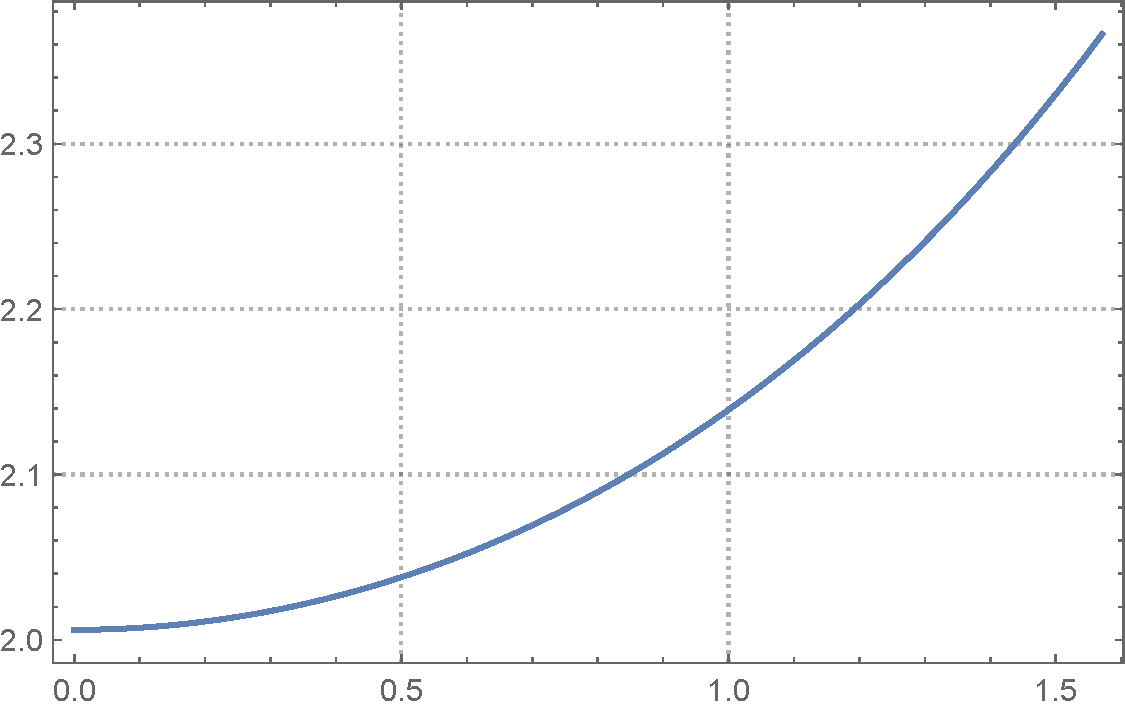
\includegraphics[width=0.8\textwidth]{Elipticky integral, Perioda}
				\captionof*{figure}{\textbf{Graf 1.}}
			\end{minipage}
			\hfill
		\end{minipage}
		\section{Numerický výpočet}
		Jak již bylo řečeno, je obtížné najít explicitní řešení rovnice ~\eqref{eq:4} ve tvaru elementárních funkcí. Programy, jako například \textit{Wolfram Mathematica}, který zde budeme využívat, ovšem umožňují rychlé nalezení numerického řešení a to hned pomocí několika numerických metod s nastavitelnými parametry.\
		\\
		\\
		Stěžejní příkaz pro výpočet numerického řešení naší diferenciální rovnice ~\eqref{eq:4} v softwaru \textit{Wolfram Mathematica} bude:
		\begin{verbatim}
			NDSolve[{\[Theta]''[t] + (g/l)*Sin[\[Theta][t]] == 0, \[Theta][0] == \[Theta]_{0}, 
				\[Theta]'[0] == 0}, \[Theta], {t,0,n}]
		\end{verbatim}
		Přičemž po celý dokument budeme ve výpočtech uvažovat délku kyvadla $ l=1 $ a gravitační zrychlení $ g=9.81 $.
		\\
		\\
		Hlavním cílem bude příkazem \textit{NDSolve} numericky určit periodu kmitů systému popsaného rovnicí ~\eqref{eq:4}, zjistit numericé řešení rovnice ~\eqref{eq:4} a prozkoumat její zachovávání/nezachovávání celkové mechanické energie během děje a všechny tyto body porovnat s reálným chováním matematického kyvadla. Výpočty budeme provádět postupně pomocí: explicitní Eulerovy metody, Rungeovy-Kuttovy metody a Symplektické Rungeovy-Kuttovy metody
		\subsection{Explicitní Eulerova metoda}
		Explicitní Eulerova metoda je jedna z jednodušších, ale ukážeme si, že také jedna z nejméně spolehlivých.
		\\
		\subsubsection{Princip explicitní Eulerovy metody.} Mějme diferenciální rovnici $\ddd{\theta}{t} + \frac{g}{l} \sin \theta = 0$ s počátečními podmínkami v čase $t_{0}=0$: $\theta(t_{0})=\theta_{0},\; \dd{\theta}{t}(t_{0})=0$. Pak řešení v čase $t_{i}=i\Delta t,\; i=1,...,n$ (zde ve vysvětlení principu předpokládáme pro zjednodušení rovnoměrné dělení a tedy $ \Delta t$ je časový krok metody) získáme ze soustavy rovnic: 
		\begin{align}
			\theta_{i+1}& =\theta_{i}+v_{i}\Delta t\\
			v_{i+1}& =v_{i}-\frac{g}{l}\sin\theta_{i}\Delta t
		\end{align}
		, kde $ v_{i}=\dd{\theta_{i}}{t},\; \theta_{i}=\theta(t_{i}),\;\theta_{i+1}=\theta(t_{i+1}),\;v_{i}=v(t_{i}),\;v_{i+1}=v(t_{i+1})$
		\\
		\subsubsection{Aproximace periody.} Nejdříve zkoumejme periodu T, kterou získáme jako 4krát dobu, za kterou se dostane kyvadlo z úhlu $\theta_{0}$ (počáteční výchylky) do úhlu $\theta=0$. 
		\\
		O takovýto výstup můžeme požádat \textit{Mathematicu} ve tvaru:  
		\begin{verbatim}
			NDSolve[{\[Theta]''[t] + g/l*Sin[\[Theta][t]] == 0, \[Theta][0] == \[Theta]_{0}, \[Theta]'[0] == 0, 
				WhenEvent[\[Theta][t] == 0, {Print[t*4], "StopIntegration"}]}, 
					\[Theta], {t, 0, n,}, Method -> "ExplicitEuler"]
		\end{verbatim}
		Důležitou vlastností matematického kyvadla je závislost periody T na počáteční výchylce $\theta_{0}$, tuto závislost ukazuje Graf 2.
		\begin{figure}[h]
			\centering
			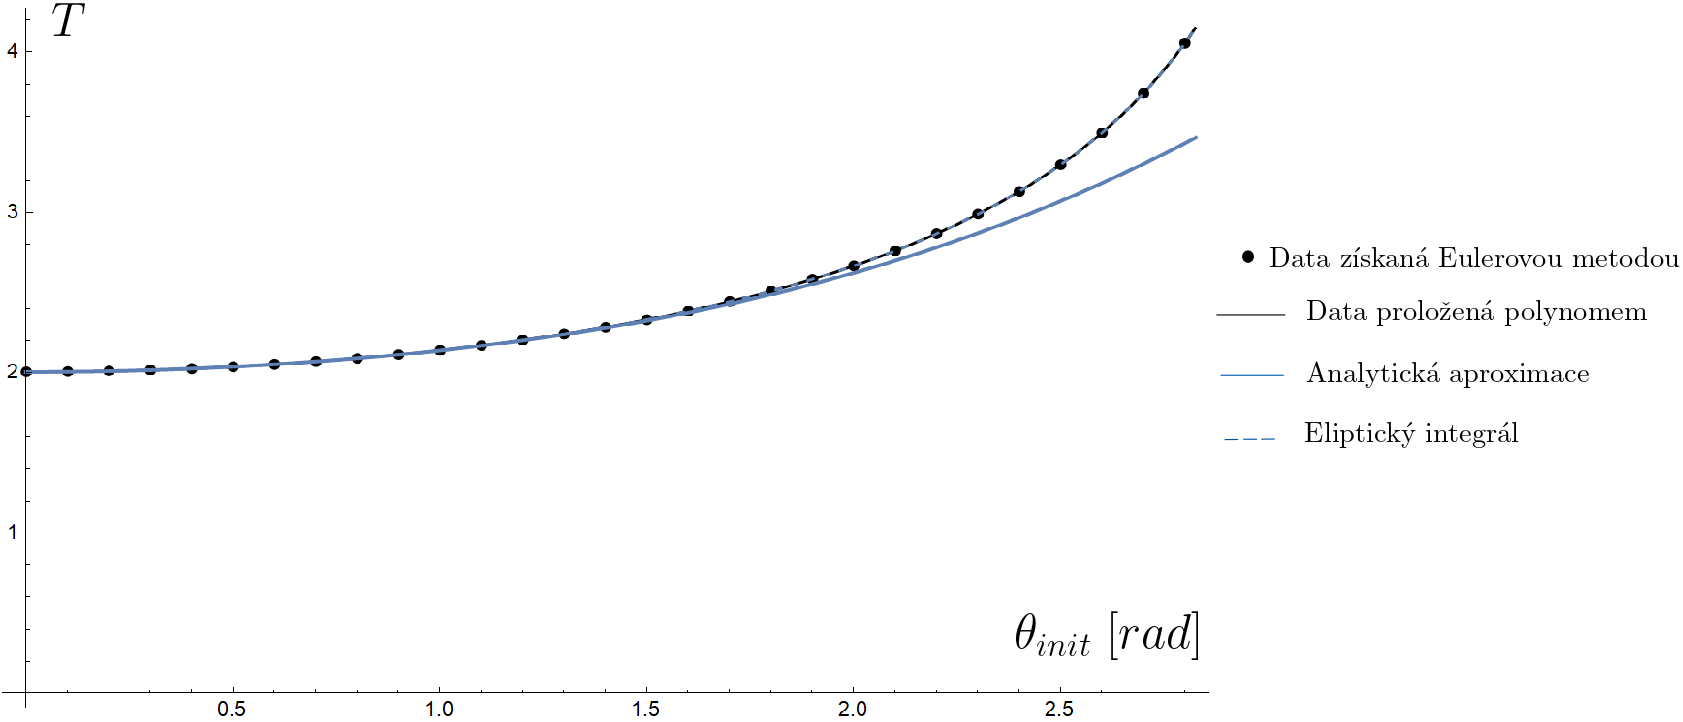
\includegraphics[width=0.8\textwidth]{graf1}
			\caption*{\textbf{Graf 2.} Závislost T na $\theta_{0}$ pro různé metody výpočtu}  
		\end{figure}
		\\
		Tečky, které jsme proložily polynomem, znázorňují hodnotu periody získané pomocí Eulerovy metody. Tyto data jsme porovnali s analityckou aproximací pomocí rovnice ~\eqref{eq:20} do 4. řádu a s výpočtem periody přes eliptický integrál, který by měl dávat přesné hodnoty.
		V tomto případě se zdá být explicitní Eulerova metoda velmi přesná. To je dáno tím, že numerické řešení pomocí explicitní Eulerovy metody se s přesných řešením rozbíhá až pro vyšší časy. Zatímco výsledky analytické aproximace jsou pro větší počáteční výchylky už i v malých časech poměrně nedostatečné.
		\\
		\\
		\subsubsection{Řešení rovnice \textit{$\ddd{\theta}{t} + \frac{g}{l} \sin \theta = 0$}.}Na grafu 3 je znázorněno řešení pohybu kyvadla vychýleného z počáteční výchylky $\theta_{0}=2\pi/3$. Modré řešení je výpočet pomocí Eulerovy metody: 
		\begin{verbatim}
		euler = NDSolve[{\[Theta]''[t] + g/l*Sin[\[Theta][t]] == 0, \[Theta][0] == \[Theta]_{0}, \[Theta]'[0] == 0,  
				\[Theta], {t, 0, n,}, Method -> "ExplicitEuler"]
		\end{verbatim}
		zároveň je zde oranžově vykresleno i řešení pomocí příkazu NDSolve, kde ale \textit{Mathematica} vybere takovou numerickou metodu, aby bylo řešení co nejpřesnější a pro nás tedy teď bude dostatečně dobrou aproximací přesných kmitů kyvadla v závisloti na čase. 
		\\
		Příkaz kterým toho dosáhneme zní:
		\begin{verbatim}
		auto = NDSolve[{\[Theta]''[t] + g/l*Sin[\[Theta][t]] == 0, 	\[Theta][0] == \[Theta]_{0}, \[Theta]'[0] == 0,  
				\[Theta], {t, 0, n,}]
		\end{verbatim}	
		Abychom tyto metody mohli porovnat, dáme je do jednoho grafu příkazem:
		\begin{verbatim}
		Plot[Evaluate[{\[Theta][t] /. euler, \[Theta][t] /. auto}], {t, 0, 100}, PlotRange -> All]
		\end{verbatim}	
		Z grafu je patrné, že Eulerova metoda pro zvyšující se \textit{t} začíná předbíhat druhé řešení a zároveň se u  této metody zvyšuje amplituda. Důvodem je v tomto případě neschopnost Eulerovy metody zachovávat celkovou mechanickou energii systému, což si ukážeme ještě lépe za chvíli.
		\begin{figure}[h]
			\centering
			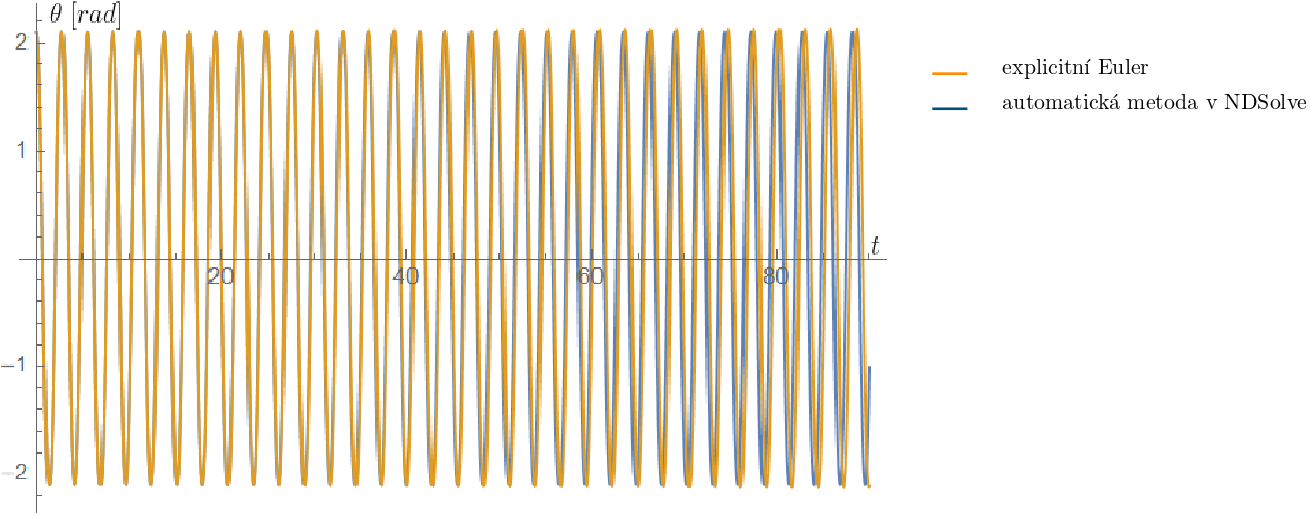
\includegraphics[width=0.9\textwidth]{vs}
			\caption*{\textbf{Graf 3.} explicitní Euler vs automatická metoda v NDSolve}  
		\end{figure}
		\\
		\\
		\subsubsection{Energie sysému.} První integrál rovnice ~\eqref{eq:4} je ve tvaru
		\begin{equation}
			\frac{1}{2}
			\left(
			\dd{\theta}{t}
			\right)^2
			-
			\frac{g}{l}
			\cos \theta
			=
			E
			.
		\end{equation}
		Což říká, že podél řešení je první integrál roven konstantě E, neboli součtu kinetické a potenciální energie, tedy dohromady celkové mechanické energii systému.
		\\
		Pro explicitní Eulerovu metodu tato rovnost ovšem neplatí. Volme například $\theta_{0} =2\pi/3$. Pro tuto počáteční výchylku by se měla zachovávat podél celého řešení celková energie $E=4.905$. Eulerova metoda ale konstantní hodnotu E nezachovává, naopak s rostoucím časem energii čím dál víc zvyšuje.
		\\
		Graf se dá vykreslit serií přikazů:
		\begin{verbatim}
		p1 = Plot[Evaluate[{((\[Theta]'[t])^2)/2 - (g/l) Cos[\[Theta][t]]} /. v], {t,0,80}, 
		PlotStyle -> Red, PlotRange -> All];
		p2 = Plot[Evaluate[-g/l *Cos[\[Theta]_{0}]], {t,0,80}, PlotRange -> All];
		Show[p1, p2, PlotRange -> All]
		\end{verbatim}
	, kde za \textit{v} dosadíme získané numerické řešení pomocí Eulerovy metody.
		\begin{figure}[h]
			\centering
			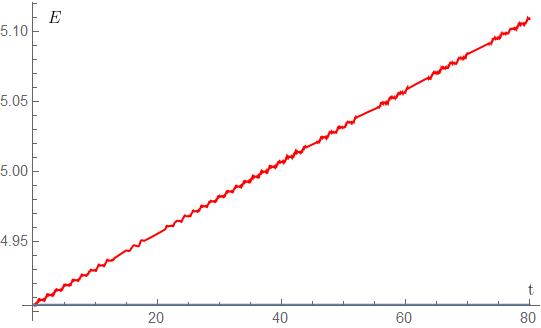
\includegraphics[width=0.72\textwidth]{energie}
			\caption*{\textbf{Graf 4.} Energie v závislosti na čase pro Eulerovu metodu.}  
		\end{figure}
		\\
		Jak moc Eulerova metoda nezachovává celkovou energie systému lze vidět z trajektorie ve vektorovém poli ${\left\lbrace \theta[t],\dd{\theta}{t}[t]\right\rbrace }$.\
		\\
		\\
		Na levém obrázku je výpočet s počáteční výchylkou $\theta_{0}=\pi/2$, kde \textit{Mathematice} přikážeme počítat Eulerovou metodou, ale nenastavíme žádné další upřesňující detaily. \textit{Mathematica} tedy sice bude počítat s obecně málo přesnou Eulerovou metodou, ale automaticky si nastaví takové parametry, aby byl výpočet co nejpřesnější.
		\\
		Během každé periody (což odpovídá jednomu oběhu ve vetorovém poli ${\left\lbrace \theta[t],\dd{\theta}{t}[t]\right\rbrace }$.) se energie pomalu zvyšuje a křivka se tak v průběhu oběhu zvětšuje. Tím pádem se ale v bodě $\left\lbrace \pi/2,0\right\rbrace $ křivka neuzavře a postupně po několika periodách vykreslí spirálu a protože se pro tento systém energie v průběhu děje zvyšuje, bude spirála pokračovvat směrem ven (výchylka kmitů se bude zvyšovat). 
		\\
		Jelikož ale toto řešení není až tak nedostatečně nepřesné, vidíme místo spirály zhušťující se křivku.
		\\
		\\
		Na pravém obrázku \textit{Mathematice} přikážeme, aby Eulerovu metodu počítala s počátečním krokem 1/99 (za metodu v příkazu NDSolve přidáme: S$ tartingStepSize -> 1/99 $). Tím se zvýší nepřesnost výpočtu a systém začne nabírat energii zřetelně rychleji.
		\begin{figure}[h]
			\centering
			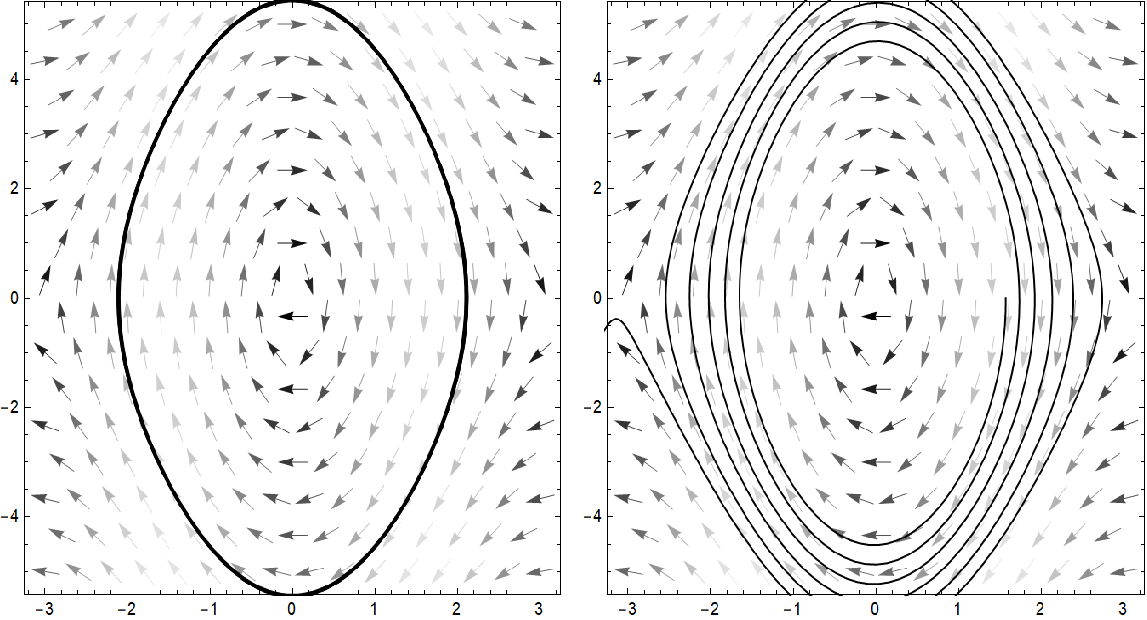
\includegraphics[width=0.72\textwidth]{pole1}
			\caption*{\textit{Nalevo:} \textbf{Obrázek 2.} automaticky zabudovaná Eulerova metoda}  \textit{Napravo:} \textbf{Obrázek 3.} Eulerova metoda s $StartingStepSize -> 1/99$  
		\end{figure}
		\clearpage
		\subsection{Rungeova-Kuttova metoda}
		\label{sec:Rungeova-Kuttova metoda}
		Rungeova-Kuttova metoda je jednokroková metoda pro numerické řešení obyčejných diferenciálních rovnic. Pro rovnici ve tvaru \( y'= f(t,y)\) s okrajovou podmínkou \(y(t_0)=y_0 \), vhodně zvolený krok \(b>0\) a \(n = 0, 1, 2, 3, ...\) , je $n+1$ krok metody definován následovně.
		\begin{align*}
			y_{n+1} &= y_n + \frac{1}{6} (k_1 + 2k_2 +2k_3 +k_4) \\
			t_{n+1} &= t_n +h \\ \\
			k_1 &= h f(t_n,y_n) \\
			k_2 &= h f\Big(t_n + \frac{h}{2},y_n + \frac{k_1}{2}\Big) \\
			k_3 &= h f\Big(t_n + \frac{h}{2},y_n + \frac{k_2}{2}\Big) \\
			k_4 &= h f(t_n + h ,y_n + k_3) 
		\end{align*}
		\subsubsection{Aproximace periody}
		\label{sec:aprox-periody}
		V následujícím jsme použily program $Mathematica$ k nalezení numerické aproximace periody kyvadla v závislosti na počáteční podmínce.
		V první části kódu jsme si zadefinovaly funkci:
		\begin{verbatim}
			Period[\[Theta]_{0}_] := (time := 0; 
			NDSolve[{\[Theta]''[t] + g/l Sin[\[Theta][t]] == 0, \[Theta][0] == \[Theta]_{0}, \[Theta]'[0] == 0, 
				WhenEvent[\[Theta][t] == 0, {time = t, "StopIntegration"}]}, \[Theta], {t, 0, 3 },
			Method -> "ExplicitRungeKutta"];
			4*time)
		\end{verbatim}
		Která na vstupu přijímá počáteční výchylku kyvadla a obratem nám vrací periodu kmitu. Pro naše potřeby jsme uvažovali tyto hodnoty konstant: $g=9.81, l=1$.\\
		Poté si stačilo nechat příkazem \verb|Table[]| s použitím naší funkce vytvořit tabulku hodnot (2). Následně jsme hodnoty metodou nejmenšího čtverce proložily polynomem a ten, společně s diskrétními hodnotami, vykreslily do grafu (2)(který?). 
		\begin{minipage}{\textwidth}
			\begin{minipage}[b]{0.25\textwidth}
				\centering
				\begin{tabular}{|c|c|}
					\hline
					$\theta_{0}$ & T \\ 
					\hline
					0.001& 2.00607\\0.101& 2.00735\\0.201& 2.01114\\0.301& 2.01749\\0.401& 2.02642\\0.501& 2.038\\0.601& 2.05231\\0.701& 2.06947\\0.801& 2.0896\\0.901& 2.11285\\1.001& 2.13942
					\\1.101& 2.16953\\1.201& 2.20344\\1.301& 2.24148\\1.401& 2.28401\\1.501& 2.33149\\
					\hline
				\end{tabular}
				\captionof*{table}{\textbf{Tabulka 2.}}
			\end{minipage}
			\begin{minipage}[b]{0.79\textwidth}
				\centering
				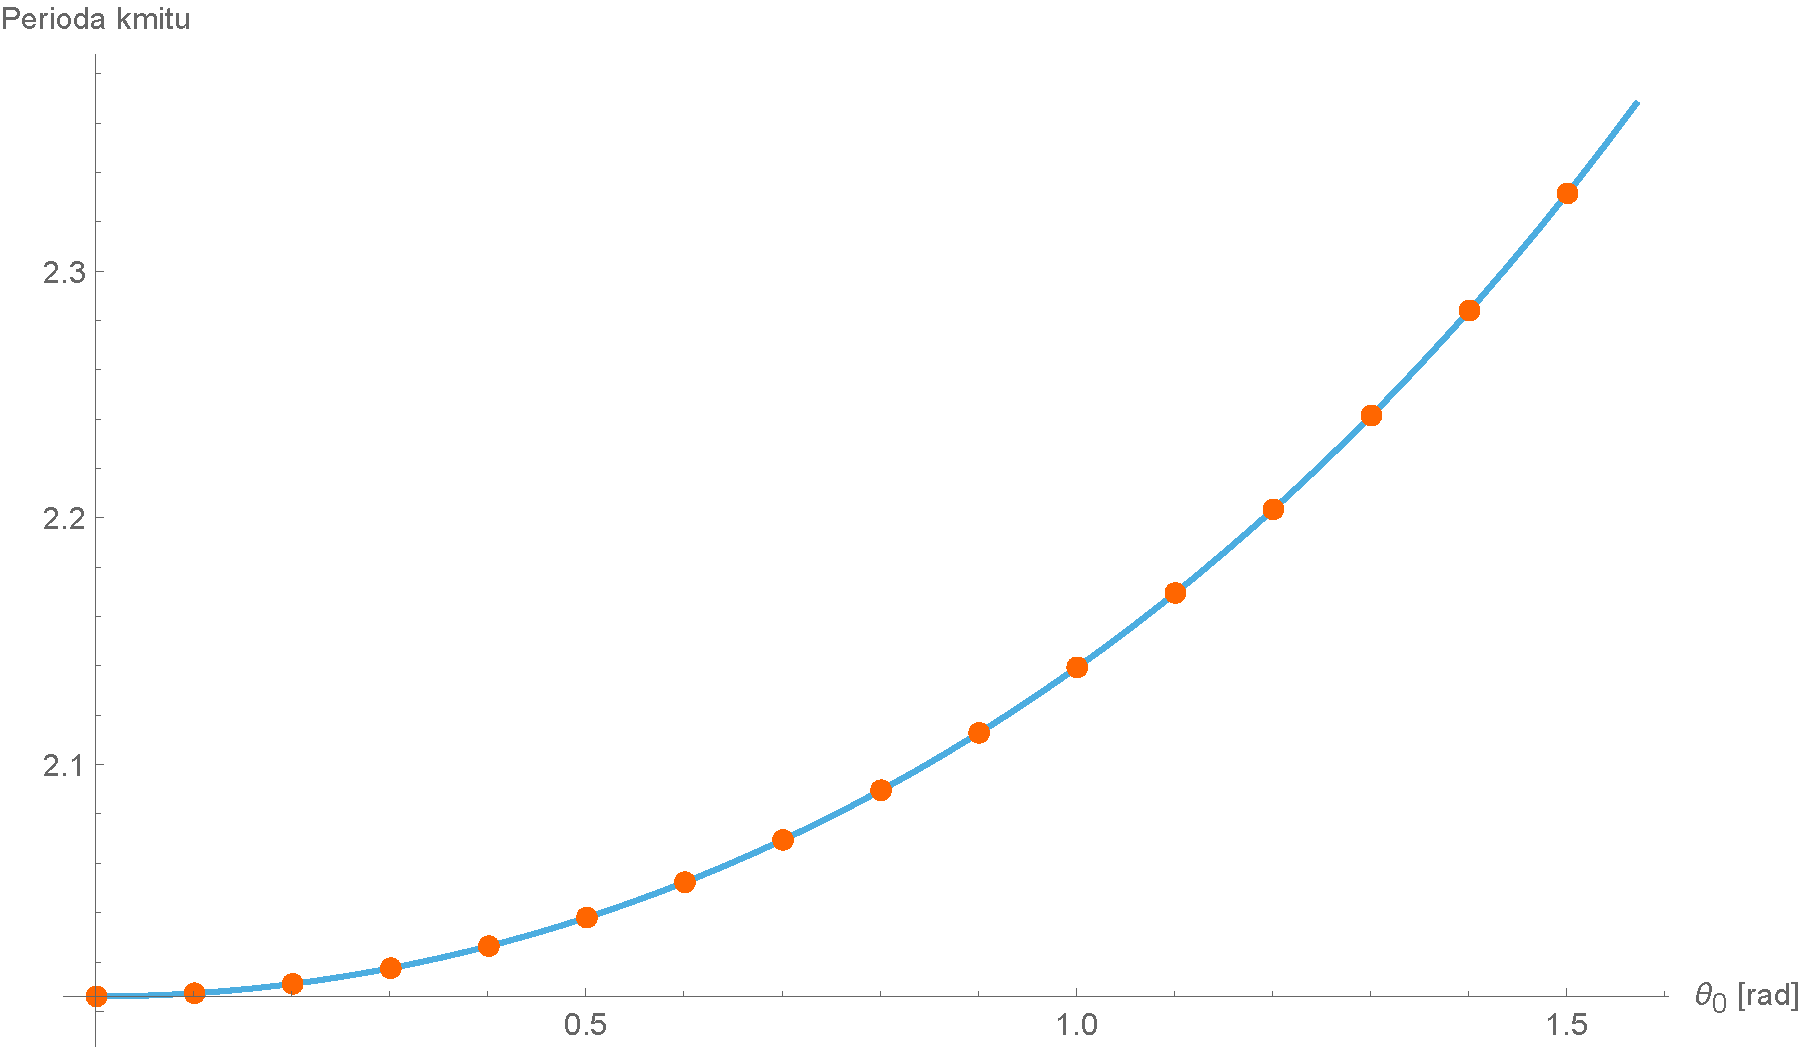
\includegraphics[width=0.8\textwidth]{Runge - Kutta, Perioda}
				\captionof*{figure}{}
			\end{minipage}
			\hfill
		\end{minipage}
		\clearpage
		\subsubsection{Energie systému}
		\label{sec:sys-energy}
		\begin{wrapfigure}{r}{5cm}
			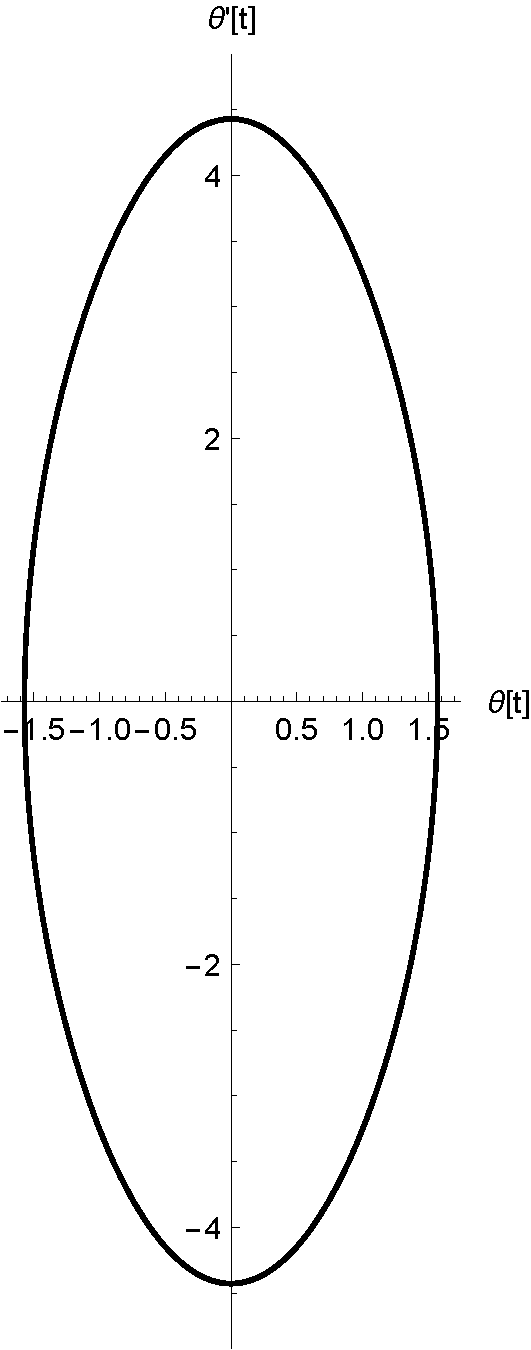
\includegraphics[width=3.5cm]{Runge - Kutta, Fazovy diagram}
			\caption*{\textbf{Obrázek 4.} Fázový diagram.}
		\end{wrapfigure}
		V této sekci zkoumáme jak dobře explicitní Rungeova-Kuttova metoda zachovává celkovou energii systému. Konkrétně se budeme zabývat počáteční podmínkou: $\theta_{0} = \pi /2$. První z vizualizací bude tzv. fázový diagram, což je parametrický graf vývoje celkové energie v čase. Na grafech tohoto typu lze velmi přímočaře identifikovat co se s energií děje. Pokud graf vypadá jako spirála, která se v čase vyvijí směrem dovnitř/ven tak celková energie systému klesá/stoupá, ale pokud se jedná o uzavřenou křivku, tak je celková energie konstatní.\\
		Pro vykreslení diagramu bylo potřeba si rovnici ~\eqref{eq:1} převést na systém rovnic prvního řádu a následně ho numericky vyřešit pro funkce \verb|x[t]|a \verb|y[t]|. Kde funkce x reprezentuje funkci $\theta [t]$ a funkce y její první derivaci (rychlost) $\theta' [t]$. Příslušný kód v Mathematice vypadá následovně:
		\begin{verbatim}
			system := NDSolve[{x'[t] == y[t], y'[t] == -g/l Sin[x[t]], x[0] == Pi/2,
				y[0] == 0}, {x[t], y[t]}, {t, 0, 10}, Method -> "ExplicitRungeKutta"]
		\end{verbatim}
		Plod naši snahy můžete nahlédnou na obrázku (2), kde nám vyšel fázový diagram uzavřený. Což znamená, že na první pohled je Rungeova-Kuttova metoda dobrá v zachovávání celkové energie.\\ \\
		K tomu jak moc dobrá v tomto metoda je, nám pomůže druhá vizualizace, kterou bude graf hodnoty celkové energie v čase. Celkovou energii získáme sečtením energie kinetické a potenciální, což v našem případě konkrétně vypadá následovně: $E = \frac{1}{2} (\theta')^2 - \frac{g}{l} cos \theta$. Takže stačí Rungeovo-Kuttovou metodou získat funkci $\theta[t]$, tu dosadit do výrazu pro $E[t]$ a funkci energie si nechat vykreslit v čase. Pro náš případ je výsledkem graf (8), z kterého jde vidět, že celková energie je skoro konstantní až na výkyvy v řádu $\pm 0.0004$.
		\begin{figure}[h]
			\begin{flushleft}
				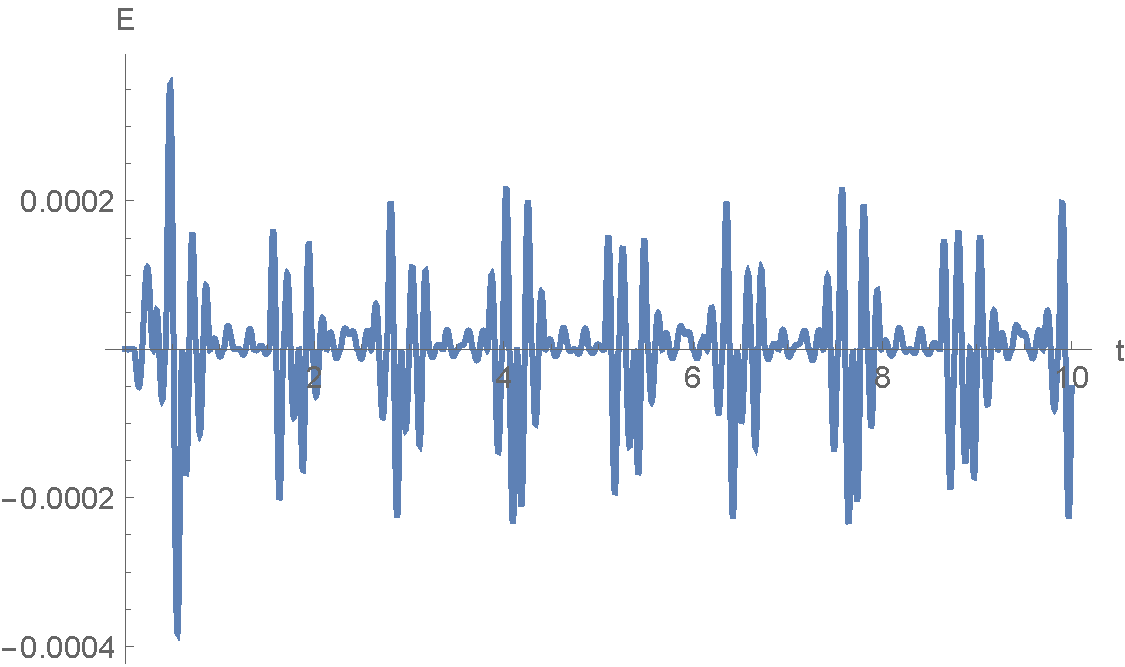
\includegraphics[width=0.65\textwidth]{Runge - Kutta, Energie}
				\caption*{\textbf{Graf 7.} Celková energie v čase}
			\end{flushleft}
		\end{figure}
		\addtocontents{toc}{\protect\end{multicols}}
\end{document}